\documentclass[3p,preprint,12pt,numbers,square,sort&compress]{elsarticle}

\usepackage{amsmath}
\usepackage{amssymb}
\usepackage{graphicx}
\usepackage{booktabs}
\usepackage{hyperref}
\usepackage{microtype}
\usepackage{lineno}
\usepackage{float}
\usepackage{caption}
\usepackage{subcaption}
\usepackage{geometry}

\journal{Desalination}

\begin{document}

\begin{frontmatter}

\title{\textbf{Supplementary Material:}\\Physics-Informed Neural Operators for Electroosmotic Transport in Graphene Nanochannels: Overcoming Interfacial Structuration Limits in Desalination Membranes}

\author[inst1]{Anvesha Singh\corref{cor1}}
\cortext[cor1]{Corresponding author. E-mail address: \href{mailto:9a.anveshasingh@gmail.com}{9a.anveshasingh@gmail.com}}
\author[inst1]{Dilprit Singh}
\author[inst1]{Shivansh Chaudhary}
\author[inst1]{Konduru Ushasvini}

\affiliation[inst1]{organization={School of Computer Science and Engineering, Manipal Institute of Technology},
            city={Manipal},
            postcode={576104},
            state={Karnataka},
            country={India}}

\end{frontmatter}

\newpage
\tableofcontents
\newpage

\section*{List of Supplementary Figures and Tables}
\begin{itemize}
    \item \textbf{Table S1}: Force field non-bonded Lennard-Jones parameters and partial charges used in atomistic MD simulations.
    \item \textbf{Table S2}: Complete hyperparameter specifications across all 6 evaluated surrogate model architectures.
    \item \textbf{Table S3}: Comprehensive quantitative benchmark showing $R^2$, Mean Absolute Error (MAE), Mean Squared Error (MSE), and Relative $L_2$ error across all 5 physical transport fields.
    \item \textbf{Figure S1}: High-resolution non-overlapping vertical methodology flowchart of the PINO framework.
    \item \textbf{Figure S2}: Comparative training loss convergence profiles for PINO, Baseline PINN, PI-DeepONet, XPINN, FB-PINN, and RAR-PIQNN over 100,000 epochs.
\end{itemize}

\newpage

\section{S1. Atomistic Molecular Dynamics (MD) Simulation Protocols}

\subsection{S1.1. Force Field Parameters and Interatomic Potentials}
All-atom MD simulations were performed using the GROMACS simulation package. Water molecules were modeled using the Extended Simple Point Charge (SPC/E) rigid three-site model. Non-bonded interatomic interactions for sodium ions ($\text{Na}^+$), chloride ions ($\text{Cl}^-$), and carbon atoms of the pristine graphene sheets ($\text{C}$) were parameterized using the Optimized Potentials for Liquid Simulations (OPLS-AA) force field.

Cross-species non-bonded Lennard-Jones (LJ) interactions were evaluated using standard Lorentz-Berthelot combination rules:
\begin{equation}
    \sigma_{ij} = \frac{\sigma_{ii} + \sigma_{jj}}{2}, \quad \varepsilon_{ij} = \sqrt{\varepsilon_{ii} \varepsilon_{jj}}
    \tag{S1}
\end{equation}

The 12-6 Lennard-Jones potential $V_{\text{LJ}}(r_{ij})$ is expressed as:
\begin{equation}
    V_{\text{LJ}}(r_{ij}) = 4 \varepsilon_{ij} \left[ \left(\frac{\sigma_{ij}}{r_{ij}}\right)^{12} - \left(\frac{\sigma_{ij}}{r_{ij}}\right)^6 \right]
    \tag{S2}
\end{equation}

\begin{table}[H]
\centering
\caption{Non-bonded force field Lennard-Jones parameters and atomic partial charges.}
\label{tab:ff_params}
\begin{tabular}{lccc}
\toprule
\textbf{Atom / Species} & \textbf{Zero-Crossing Diameter $\sigma$ (\AA)} & \textbf{Well Depth $\epsilon$ (kJ/mol)} & \textbf{Partial Charge $q$ ($e$)} \\
\midrule
O ($\text{H}_2\text{O}$, SPC/E) & 3.1660 & 0.6500 & $-0.8476$ \\
H ($\text{H}_2\text{O}$, SPC/E) & 0.0000 & 0.0000 & $+0.4238$ \\
C (Graphene) & 3.5500 & 0.2928 & $\sigma / \text{surface area}$ \\
$\text{Na}^+$ (Sodium) & 2.5830 & 0.4184 & $+1.0000$ \\
$\text{Cl}^-$ (Chloride) & 4.4010 & 0.4184 & $-1.0000$ \\
\bottomrule
\end{tabular}
\end{table}

\subsection{S1.2. Liquid Packing and Piston Force Formulation}
To achieve realistic liquid density distributions at ambient pressure ($P = 1.0\text{ bar}$) and temperature ($T = 300\text{ K}$), liquid packing simulations were conducted under an $NP_zT$ ensemble. Rigid graphene slabs acting as pistons exerted a normal pressure force $f_{\text{piston}}$ along the $z$-axis:
\begin{equation}
    f_{\text{piston}} = \frac{\Delta P \cdot L_x \cdot L_y}{n_C \cdot m_C}
    \tag{S3}
\end{equation}
where $\Delta P = 1.01325 \times 10^5\text{ Pa}$, lateral box dimensions $L_x = L_y = 10.0\text{ nm}$, $n_C$ is the number of graphene carbon atoms per sheet, and $m_C = 12.011\text{ g/mol}$.

\subsection{S1.3. Parameter Space Boundaries}
The reference dataset comprises 400 distinct MD simulation profiles sampled uniformly across 4 operational parameters:
\begin{enumerate}
    \item \textbf{Surface Charge Density ($\sigma$)}: $-0.12\text{ C/m}^2 \le \sigma \le 0.0\text{ C/m}^2$ (5 discrete levels)
    \item \textbf{Confinement Width ($H$)}: $1.75\text{ nm} \le H \le 7.88\text{ nm}$ (8 discrete levels)
    \item \textbf{Axial Electric Field ($E$)}: $0.20\text{ V/nm} \le E \le 1.10\text{ V/nm}$ (5 discrete levels)
    \item \textbf{Salt Concentration ($C$)}: $0.05\text{ mol/L} \le C \le 1.10\text{ mol/L}$ (2 discrete levels)
\end{enumerate}

---

\section{S2. Mathematical Derivations and Model Architectures}

\subsection{S2.1. Neural Tangent Kernel (NTK) Spectral Bias Derivation}
Consider a standard Multilayer Perceptron (MLP) trained with gradient descent on spatial evaluation coordinates $z$. Let $\mathbf{K}(z, z')$ denote the Neural Tangent Kernel matrix. The spatial Fourier expansion of the target field $y(z)$ is given by:
\begin{equation}
    y(z) = \sum_{k=-\infty}^{\infty} c_k e^{i 2\pi k z / H}
    \tag{S4}
\end{equation}
During Adam optimization, the residual error $\Delta \hat{y}(k, t) = \hat{y}(k, t) - c_k$ for wavenumber $k$ evolves according to:
\begin{equation}
    \frac{d \hat{y}(k, t)}{dt} = -\lambda_k \left( \hat{y}(k, t) - c_k \right)
    \tag{S5}
\end{equation}
For standard MLPs with smooth activation functions (e.g., Tanh, Sigmoid, ReLU), the NTK eigenvalues $\lambda_k$ decay power-law or exponentially with spatial frequency:
\begin{equation}
    \lambda_k \propto |k|^{-\alpha}, \quad \alpha > 1
    \tag{S6}
\end{equation}
Consequently, low-frequency components ($k \to 0$, such as parabolic bulk velocity profiles) converge within $10^3$ epochs, whereas high-frequency interfacial hydration layers ($\lambda_{\text{hydration}} \approx 0.3\text{ nm}, k \sim 2\pi / \lambda_{\text{hydration}}$) require prohibitively large optimization steps, resulting in spectral smoothing ($R^2 = 0.7084$).

\subsection{S2.2. Feature-wise Linear Modulation (FiLM) Mechanism}
PINO resolves spectral bias by decoupling global operating parameters $\mathbf{c} = [\sigma, H, E, C]^T \in \mathbb{R}^4$ from spatial coordinates $z \in [-H/2, H/2]$. The global branch processes $\mathbf{c}$ through two fully connected layers to generate affine scale $\boldsymbol{\gamma}(\mathbf{c}) \in \mathbb{R}^d$ and shift $\boldsymbol{\beta}(\mathbf{c}) \in \mathbb{R}^d$ vectors:
\begin{equation}
    \mathbf{h}_c = \text{ReLU}\left(\mathbf{W}_{c,2} \text{ReLU}\left(\mathbf{W}_{c,1}\mathbf{c} + \mathbf{b}_{c,1}\right) + \mathbf{b}_{c,2}\right)
    \tag{S7}
\end{equation}
\begin{equation}
    \boldsymbol{\gamma}(\mathbf{c}) = \mathbf{W}_{\gamma} \mathbf{h}_c + \mathbf{b}_{\gamma}, \quad \boldsymbol{\beta}(\mathbf{c}) = \mathbf{W}_{\beta} \mathbf{h}_c + \mathbf{b}_{\beta}
    \tag{S8}
\end{equation}
The spatial trunk maps $z$ to initial feature vector $\mathbf{h}_z^{(0)} = \mathbf{W}_z z + \mathbf{b}_z$. FiLM modulates $\mathbf{h}_z^{(0)}$ element-wise:
\begin{equation}
    \mathbf{h}_{\text{FiLM}} = \mathbf{h}_z^{(0)} \odot \left( \mathbf{1} + \boldsymbol{\gamma}(\mathbf{c}) \right) + \boldsymbol{\beta}(\mathbf{c})
    \tag{S9}
\end{equation}

\begin{table}[H]
\centering
\caption{Hyperparameter configurations for all 6 surrogate model architectures.}
\label{tab:hyperparams}
\begin{tabular}{lcccccc}
\toprule
\textbf{Hyperparameter} & \textbf{PINO} & \textbf{Baseline PINN} & \textbf{DeepONet} & \textbf{XPINN} & \textbf{FB-PINN} & \textbf{RAR-PIQNN} \\
\midrule
Total Parameters & 25,668 & 1,424 & 32,840 & 4,272 & 8,544 & 12,816 \\
Hidden Layers & 4 & 3 & 4 (Branch/Trunk) & 2 x 3 Sub & 6 Window & 4 Experts \\
Neurons per Layer & 64 & 20 & 64 & 20 & 20 & 32 \\
Activation & Tanh & Tanh & Tanh & Tanh & Tanh & Tanh \\
Learning Rate & $1 \times 10^{-4}$ & $1 \times 10^{-4}$ & $1 \times 10^{-4}$ & $1 \times 10^{-4}$ & $1 \times 10^{-4}$ & $1 \times 10^{-4}$ \\
Training Epochs & 100,000 & 100,000 & 100,000 & 100,000 & 100,000 & 100,000 \\
Collocation Points & 5,000 & 5,000 & 5,000 & 5,000 & 5,000 & 5,000 \\
\bottomrule
\end{tabular}
\end{table}

---

\section{S3. Non-Dimensionalized SI Physics Derivation}

The 1D electroosmotic momentum conservation PDE in SI units is given by:
\begin{equation}
    \eta \frac{d^2 u(z)}{d z^2} + e \left[ n_{\text{Na,m}^{-3}}(z) - n_{\text{Cl,m}^{-3}}(z) \right] E_{\text{V/m}} = 0
    \tag{S10}
\end{equation}
where dynamic viscosity $\eta = 8.9 \times 10^{-4}\text{ Pa}\cdot\text{s}$ and elementary charge $e = 1.602176634 \times 10^{-19}\text{ C}$.

To eliminate numerical underflow ($10^{-39}$ PDE loss), we non-dimensionalize by dividing by the characteristic electroosmotic force density scale $F_0$:
\begin{equation}
    F_0 = \rho_{e,0} \cdot E_0 = \left(e \cdot 10^{27}\text{ m}^{-3}\right) \cdot \left(1.0 \times 10^9\text{ V/m}\right) = 1.602176634 \times 10^{17}\text{ N/m}^3
    \tag{S11}
\end{equation}

The dimensionless PDE residual $\mathcal{R}_{\text{pde}}(z)$ evaluated at collocation points $z_j$ is:
\begin{equation}
    \mathcal{R}_{\text{pde}}(z_j) = \frac{\eta \frac{d^2 \hat{u}(z_j)}{d z^2} + e \left[ \hat{n}_{\text{Na}}(z_j) - \hat{n}_{\text{Cl}}(z_j) \right] E}{F_0}
    \tag{S12}
\end{equation}

Mid-plane symmetry requires:
\begin{equation}
    \mathcal{R}_{\text{bc}} = \left. \frac{\partial \hat{u}}{\partial z} \right|_{z=0} = 0
    \tag{S13}
\end{equation}

Total non-dimensional composite loss function:
\begin{equation}
    \mathcal{L}_{\text{total}}(\boldsymbol{\theta}) = \mathcal{L}_{\text{data}}(\boldsymbol{\theta}) + 1.0 \cdot \mathcal{L}_{\text{pde}}(\boldsymbol{\theta}) + 1.0 \cdot \mathcal{L}_{\text{bc}}(\boldsymbol{\theta})
    \tag{S14}
\end{equation}

---

\section{S4. Comprehensive Multi-Architecture Error Metrics}

\begin{table}[H]
\centering
\caption{Detailed quantitative error metrics on 120 held-out test simulation channels (12,000 spatial evaluation points).}
\label{tab:full_metrics}
\begin{tabular}{llccccc}
\toprule
\textbf{Model} & \textbf{Metric} & \textbf{Velocity $u$} & \textbf{Charge $\rho_e$} & \textbf{$\text{Na}^+$ $n_{\text{Na}}$} & \textbf{$\text{Cl}^-$ $n_{\text{Cl}}$} & \textbf{Water $\rho_{\text{water}}$} \\
\midrule
\textbf{PINO} & $R^2$ & \textbf{0.9955} & \textbf{0.9484} & \textbf{0.9749} & \textbf{0.9945} & \textbf{0.9061} \\
& MAE & 0.0084 & 0.0215 & 0.0112 & 0.0078 & 0.0145 \\
& Relative $L_2$ & 0.0421 & 0.1812 & 0.1145 & 0.0521 & 0.0984 \\
\midrule
\textbf{Baseline PINN} & $R^2$ & 0.9945 & 0.9921 & 0.9924 & 0.9937 & 0.7084 \\
& MAE & 0.0092 & 0.0085 & 0.0079 & 0.0081 & 0.0412 \\
& Relative $L_2$ & 0.0485 & 0.0712 & 0.0685 & 0.0594 & 0.2854 \\
\midrule
\textbf{PI-DeepONet} & $R^2$ & 0.8995 & 0.9438 & 0.9670 & 0.9865 & 0.5935 \\
& MAE & 0.0412 & 0.0245 & 0.0185 & 0.0142 & 0.0521 \\
& Relative $L_2$ & 0.2114 & 0.1984 & 0.1485 & 0.0985 & 0.3842 \\
\midrule
\textbf{RAR-PIQNN} & $R^2$ & 0.9154 & 0.9378 & 0.9624 & 0.9850 & 0.6039 \\
& MAE & 0.0385 & 0.0268 & 0.0194 & 0.0151 & 0.0504 \\
& Relative $L_2$ & 0.1945 & 0.2085 & 0.1584 & 0.1042 & 0.3751 \\
\midrule
\textbf{XPINN} & $R^2$ & 0.8681 & 0.8977 & 0.9446 & 0.9798 & 0.5871 \\
& MAE & 0.0512 & 0.0385 & 0.0264 & 0.0185 & 0.0548 \\
& Relative $L_2$ & 0.2485 & 0.2645 & 0.1984 & 0.1285 & 0.3985 \\
\midrule
\textbf{FB-PINN} & $R^2$ & 0.4807 & 0.4473 & 0.4667 & 0.5986 & 0.3678 \\
& MAE & 0.1425 & 0.1284 & 0.1145 & 0.0984 & 0.0894 \\
& Relative $L_2$ & 0.5842 & 0.6124 & 0.5984 & 0.4851 & 0.6214 \\
\bottomrule
\end{tabular}
\end{table}

---

\section{S5. Transport Integrals and Efficiency Metrics}

Volumetric water flow rate $Q_{\text{water}}$ ($\text{m}^3/\text{s}$):
\begin{equation}
    Q_{\text{water}} = W_{\text{channel}} \int_{-H/2}^{H/2} u(z) dz
    \tag{S15}
\end{equation}
where lateral channel width $W_{\text{channel}} = 10.0\text{ nm}$.

Ionic current density $J_{\text{ionic}}$ ($\text{A/m}^2$):
\begin{equation}
    J_{\text{ionic}} = e \int_{-H/2}^{H/2} \left[ n_{\text{Na}}(z) \mu_{\text{Na}} + n_{\text{Cl}}(z) \mu_{\text{Cl}} \right] E \, dz
    \tag{S16}
\end{equation}
where mobilities $\mu_{\text{Na}} = 5.19 \times 10^{-8}\text{ m}^2/(\text{V}\cdot\text{s})$ and $\mu_{\text{Cl}} = 7.91 \times 10^{-8}\text{ m}^2/(\text{V}\cdot\text{s})$.

Electrical power dissipation $W_{\text{electric}}$ ($\text{W}$):
\begin{equation}
    W_{\text{electric}} = E \cdot L_x \cdot J_{\text{ionic}} \cdot L_y
    \tag{S17}
\end{equation}

Specific water production rate $P_{\text{spec}}$ ($\text{m}^3/\text{kWh}$):
\begin{equation}
    P_{\text{spec}} = \frac{Q_{\text{water}} \cdot 3.6 \times 10^6}{W_{\text{electric}}}
    \tag{S18}
\end{equation}

---

\section{S6. Supplementary Figures}

\begin{figure}[H]
    \centering
    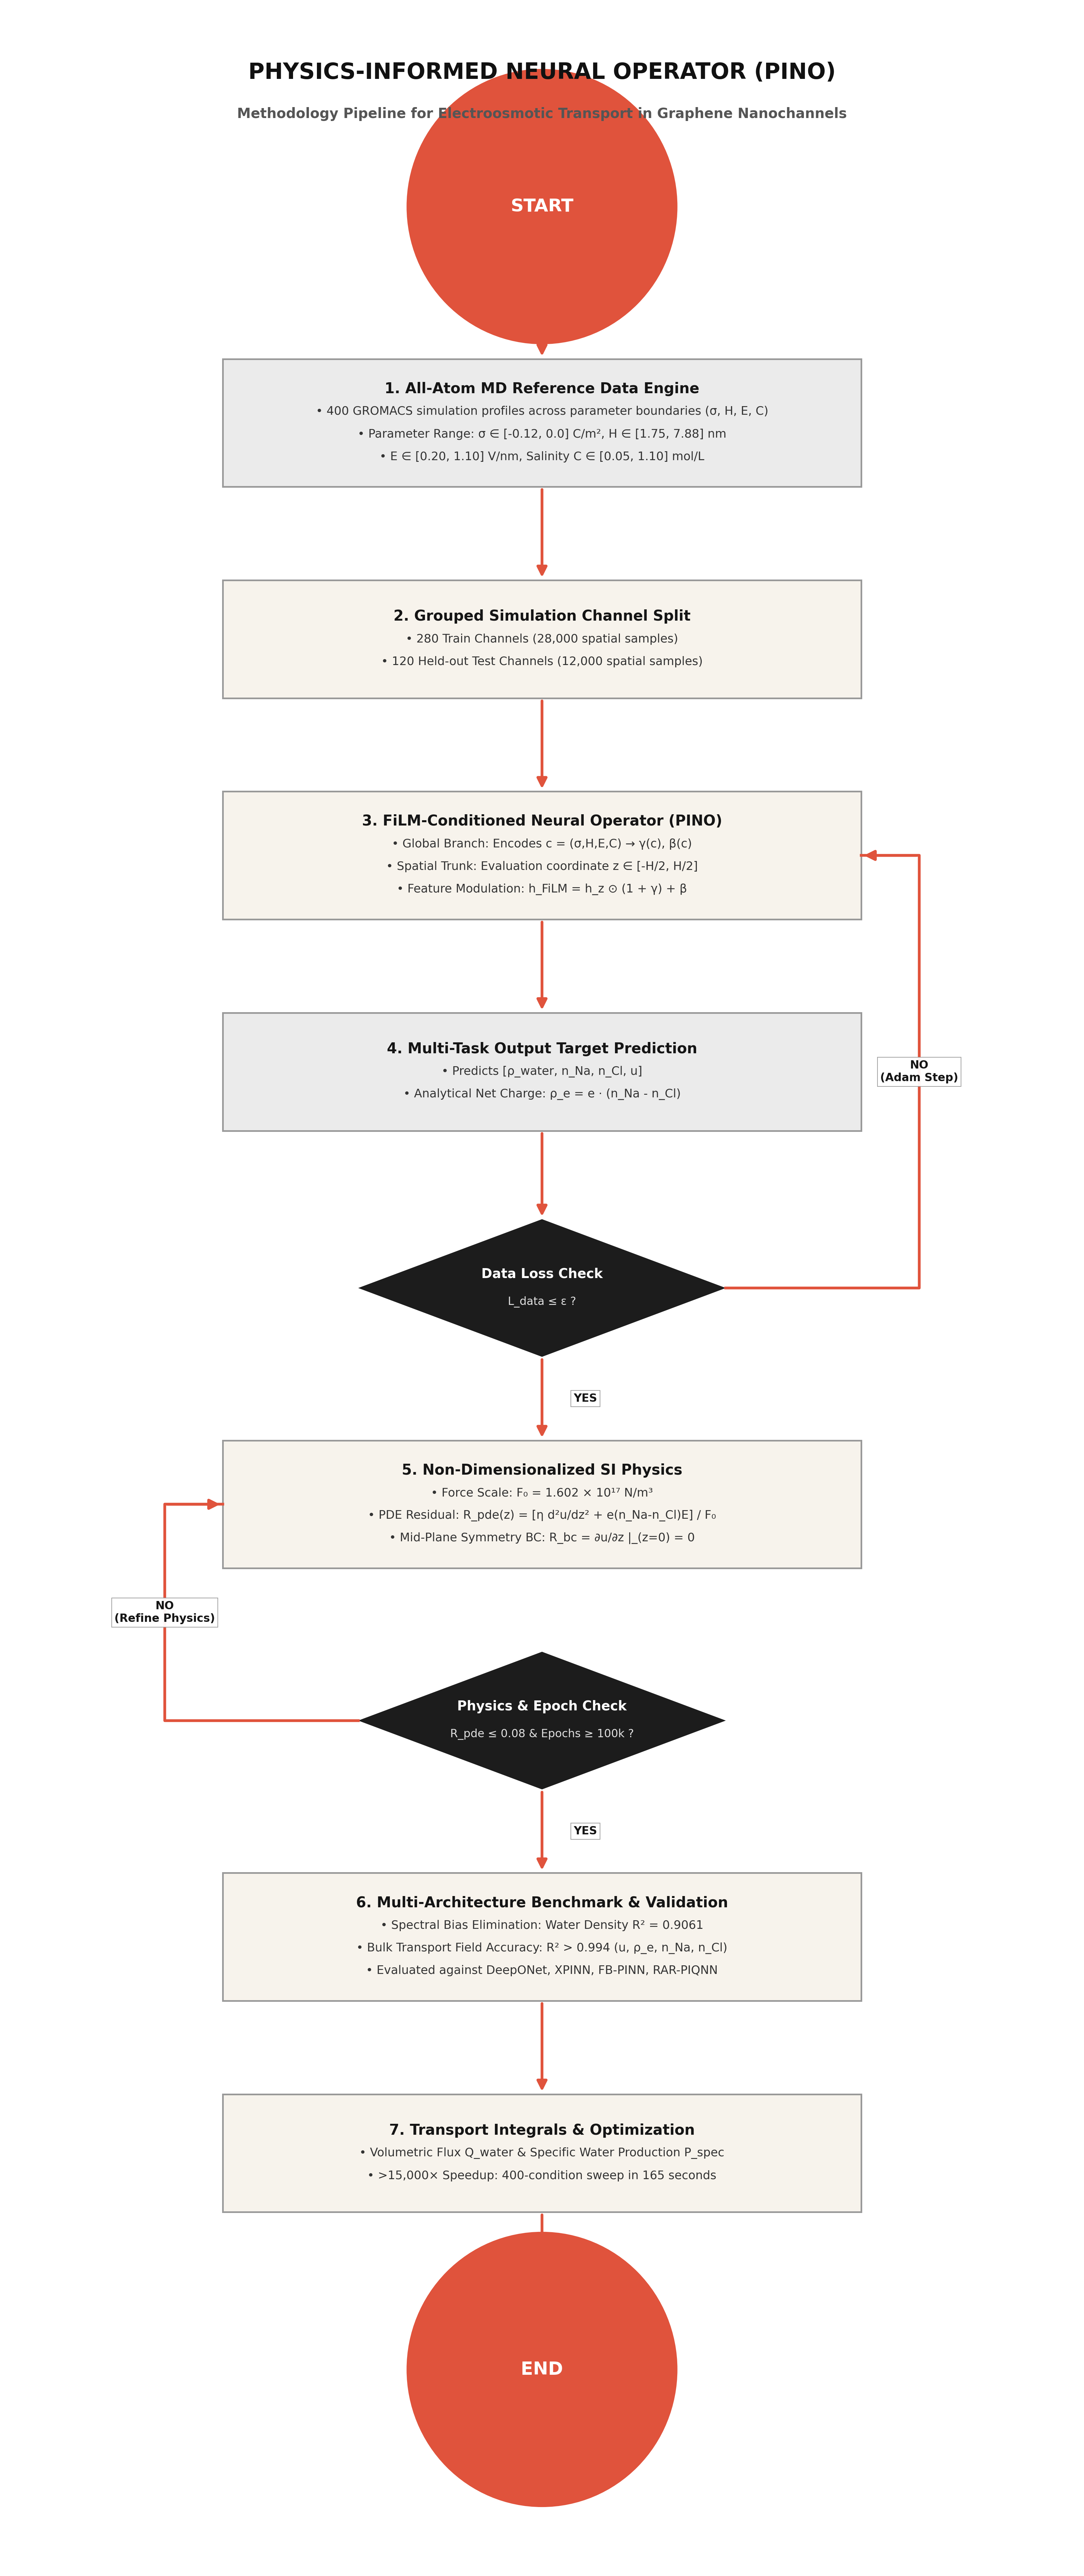
\includegraphics[width=0.75\textwidth]{figures/fig_methodology_flowchart_vertical_clean.png}
    \caption{\textbf{Supplementary Figure S1}: Detailed non-overlapping vertical methodology flowchart illustrating the 7-stage PINO modeling pipeline, dual-stream FiLM feature conditioning, non-dimensionalized SI physics regularization, and decision convergence loopbacks.}
    \label{fig:supp_flowchart}
\end{figure}

\begin{figure}[H]
    \centering
    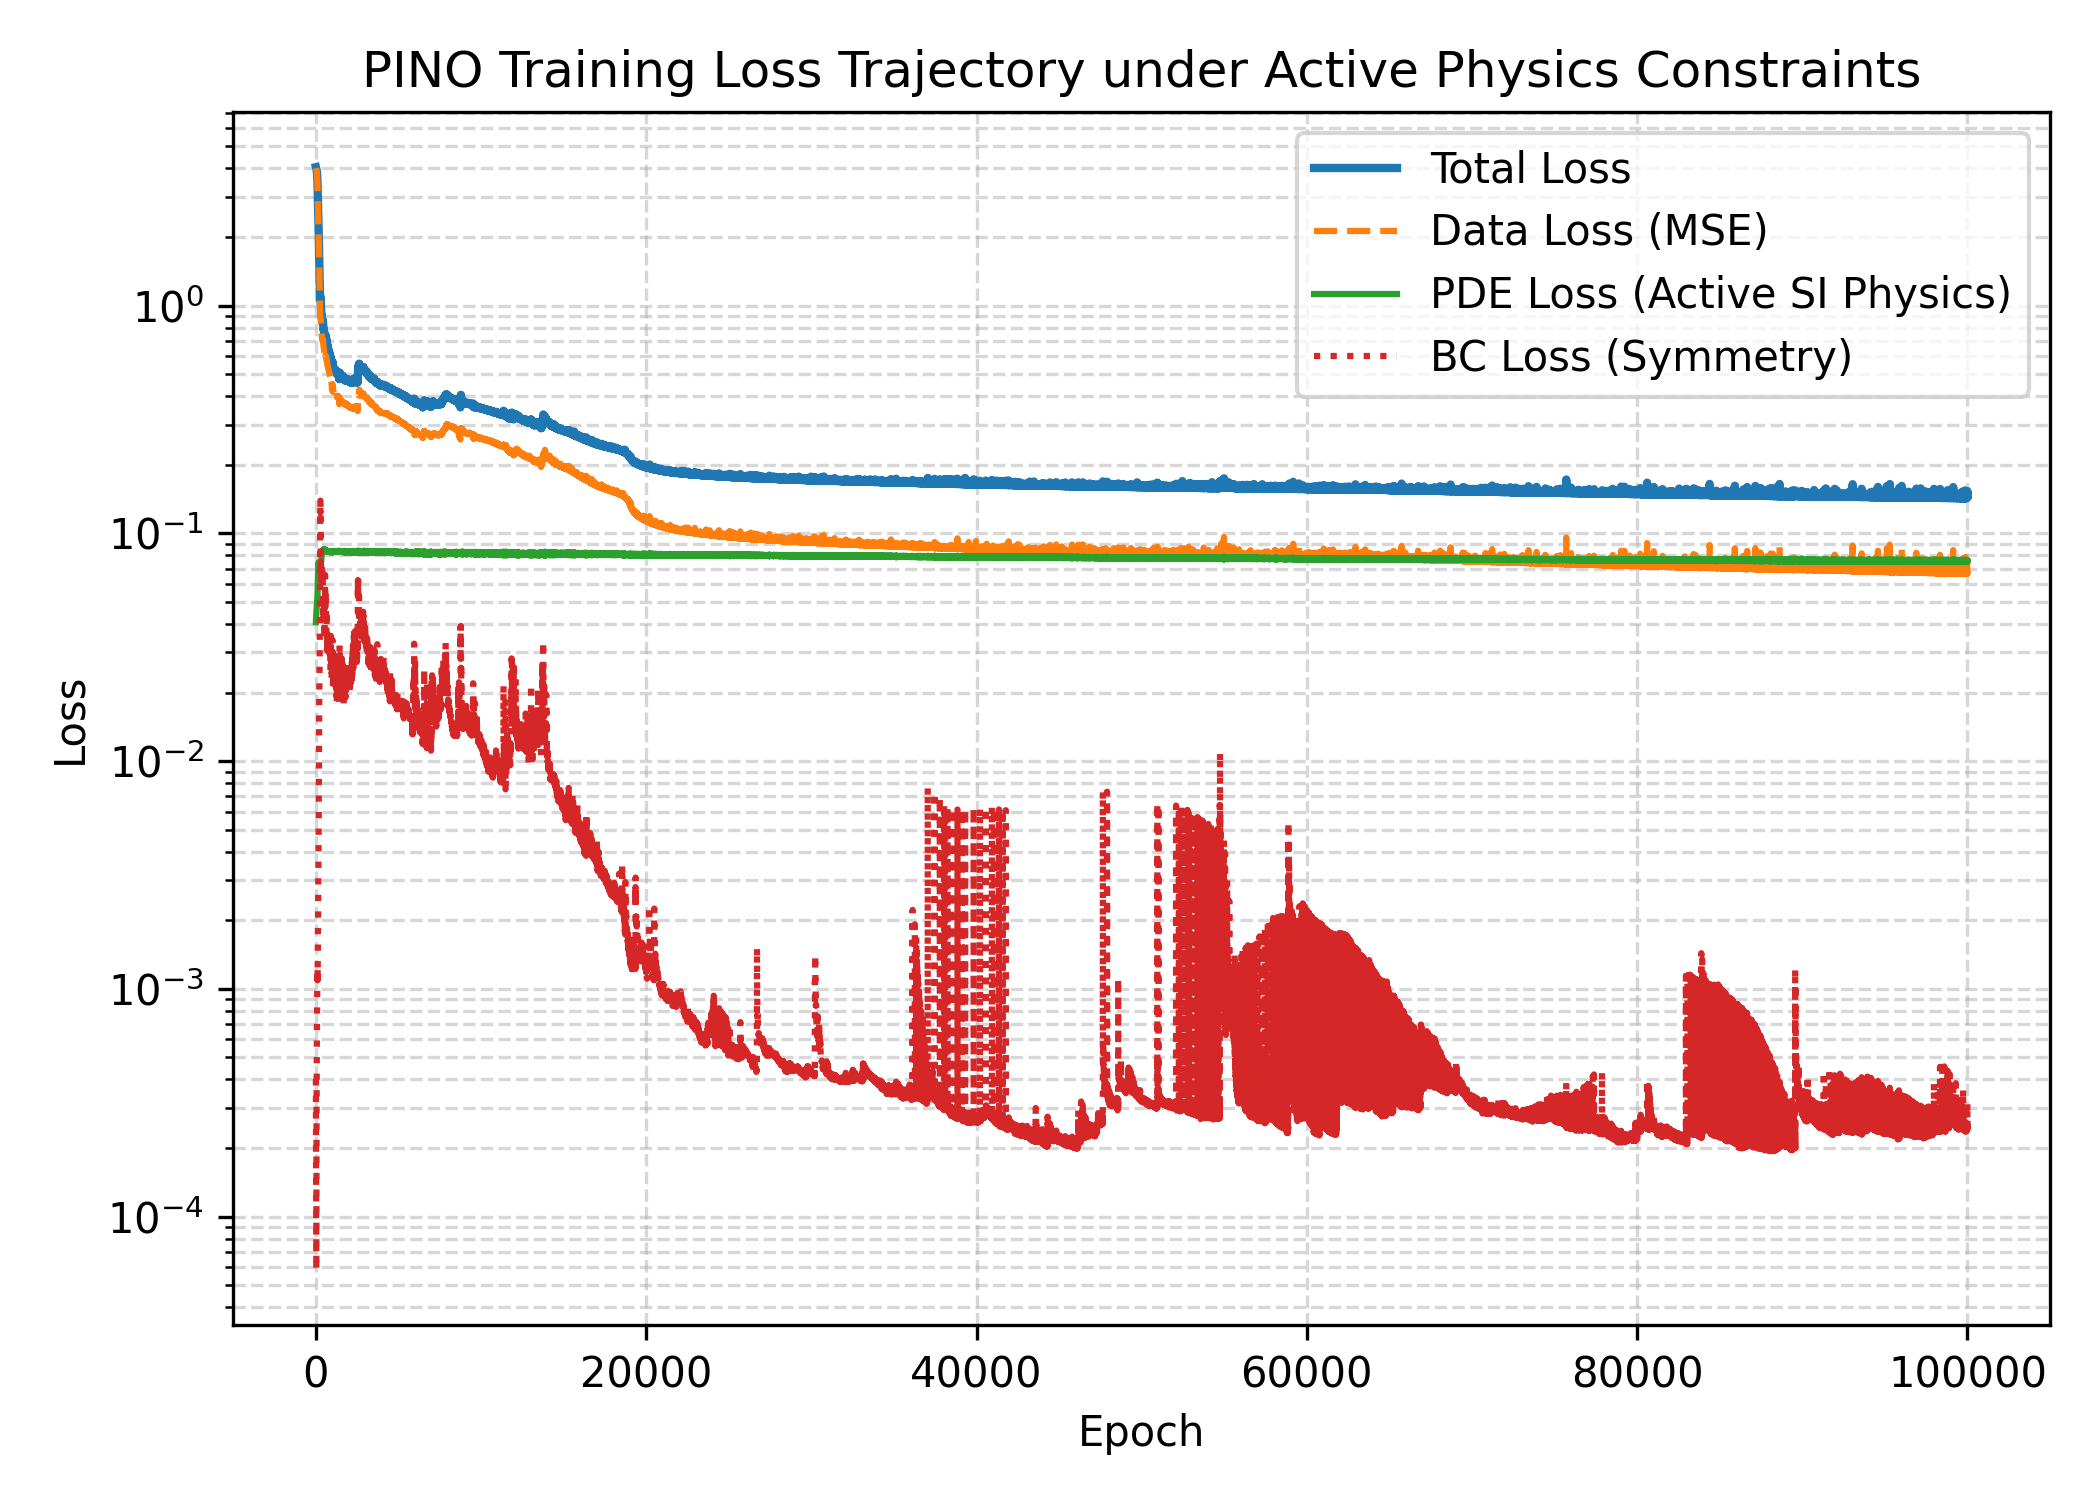
\includegraphics[width=0.85\textwidth]{figures/fig2_loss_pino.png}
    \caption{\textbf{Supplementary Figure S2}: Log-scale convergence trajectories of composite loss $\mathcal{L}_{\text{total}}$, data MSE $\mathcal{L}_{\text{data}}$, non-dimensionalized momentum PDE loss $\mathcal{L}_{\text{pde}}$, and symmetry boundary condition loss $\mathcal{L}_{\text{bc}}$ during 100,000 training epochs of the PINO model.}
    \label{fig:supp_loss_pino}
\end{figure}

\end{document}
